\documentclass[handout]{beamer}
\usetheme{Boadilla}
\usepackage[backend=biber,style=numeric-comp,isbn=true]{biblatex}

\addbibresource{RelatedWork.bib}
\setbeamercolor*{bibliography entry title}{parent=palette primary}

\usepackage{mathpartir}
\usepackage{listings}
\usepackage{tikz}
\usepackage{wasysym}
\usepackage{xcolor}
\usepackage{amsmath}
\usepackage{scalerel}

\usetikzlibrary{arrows.meta,
                chains,
                positioning,
                shapes.geometric
                }

\lstdefinelanguage{dtt}{
    keywords={contract, library, function, public, storage, memory, msg, sender, payable, return, revert, if, event, indexed, external, emit},
    keywordstyle=\color{blue}\bfseries,
    ndkeywords={uint, address, bool, mapping, bytes, uint256},
    ndkeywordstyle=\color{purple},
    identifierstyle=\color{black},
    sensitive=false,
    comment=[l]{//},
    morecomment=[s]{(*}{*)},
    commentstyle=\color{brown}\ttfamily,
    stringstyle=\color{red}\ttfamily,
    morestring=[b]',
    morestring=[b]",
    showstringspaces=false,
    literate={->}{$\rightarrow\ $}1
}

\lstset{
    basicstyle=\ttfamily\tiny,
    language=dtt
}
\newcommand{\code}[1]{\lstinline!#1!}
\newcommand{\colorcite}[2]{\textcolor{blue}{\cite[#1]{#2}}}
\newcommand{\always}{\textcolor{red}{\text{ALWAYS }}}
\newcommand{\nextt}{\textcolor{red}{\text{NEXT }}}
\newcommand{\even}{\textcolor{red}{\text{EVENTUALLY }}}
\newcommand{\alwaysf}{\Box}
\newcommand{\nexttf}{\mathcal{X}}
\newcommand{\evenf}{\Diamond}
\newcommand{\stronguntil}{\hspace{0.1cm} \mathcal{U}  \hspace{0.1cm}}
\newcommand{\strongrelease}{\hspace{0.1cm} \mathcal{M} \hspace{0.1cm}}
\newcommand{\weakuntil}{\hspace{0.1cm} \mathcal{W} \hspace{0.1cm}}
\newcommand{\weakrelease}{\hspace{0.1cm} \mathcal{R} \hspace{0.1cm}}
\newcommand{\Buchi}{B\"{u}chi }
\newcommand{\limplies}{\rightarrow}
\newcommand{\liff}{\leftrightarrow}
\DeclareMathOperator*{\bigplus}{\scalerel*{+}{\sum}}

% section slides
\AtBeginSection[]{
  \begin{frame}
  \vfill
  \centering
  \begin{beamercolorbox}[sep=8pt,center,shadow=true,rounded=true]{title}
    \usebeamerfont{title}\insertsectionhead\par%
  \end{beamercolorbox}
  \vfill
  \end{frame}
}

\makeatother
\setbeamertemplate{footline}
{
  \leavevmode%
  \hbox{%
  \begin{beamercolorbox}[wd=.333333\paperwidth,ht=2.25ex,dp=1ex,center]{author in head/foot}%
    \usebeamerfont{author in head/foot}\insertshortauthor%~~(\insertshortinstitute)
  \end{beamercolorbox}%
  \begin{beamercolorbox}[wd=.333333\paperwidth,ht=2.25ex,dp=1ex,center]{title in head/foot}%
    \usebeamerfont{title in head/foot} Linear Temporal Logic Visualization
  \end{beamercolorbox}%
  \begin{beamercolorbox}[wd=.333333\paperwidth,ht=2.25ex,dp=1ex,right]{date in head/foot}%
    \usebeamerfont{date in head/foot}\insertshortdate{}\hspace*{2em}
    \insertframenumber{} / \inserttotalframenumber\hspace*{2ex}
  \end{beamercolorbox}}%
  \vskip0pt%
}
\makeatletter


\title{What's in a Name? Linear Temporal Logic Literally Represents Time Lines}
\subtitle{Project Report for 15-816}
\author{Runming Li \& Keerthana Gurushankar}
\institute[]{Carnegie Mellon University \\ \{runmingl, kgurusha\}@andrew.cmu.edu\\
Mentored by Kristin Yvonne Rozier \& Marijn Heule}
\date{December 14, 2022}

\begin{document}
\maketitle

\begin{frame}{What is LTL?}
    \begin{align*}
        a ::= & p \mid q \mid r \mid \cdots \tag{atomic propositions} \\
        \Phi ::= & a \tag{atomic} \\
        \mid & \neg \Phi \tag{negation} \\ 
        \mid & \Phi \vee \Phi \tag{disjunction} \\
        \mid & \Phi \wedge \Phi \tag{conjunction} \\
        \mid & \Phi \rightarrow \Phi \tag{implication} \\
        \mid & \alwaysf \Phi \tag{always} \\
        \mid & \evenf \Phi \tag{eventually} \\
        \mid & \nexttf \Phi \tag{next}
    \end{align*}
    $\alwaysf \Phi = \Phi$ is \always true \\
    $\evenf \Phi = \Phi$ is \even true \\
    $\nexttf \Phi = \Phi$ is true in the \nextt time step\footnote{Other temporal connectives untils ($\stronguntil, \weakuntil$) and releases ($\strongrelease, \weakrelease$) are omitted} 
\end{frame}

\begin{frame}{Can you tell the difference?\footnote{slide adapted from Rozier}}
A NASA Rocket Scientist was given this English specification:

``\textbf{p oscillates every time step}''

She wrote two possible LTL formulas:
\[
    \Phi = \always ((p \wedge \nextt \neg p) \vee (\neg p \wedge \nextt p))
\]
\[
    \Psi = \always ((p \wedge \nextt \neg p) \wedge (\neg p \wedge \nextt p))
\]

Which one is correct?    
\end{frame}

\begin{frame}{Which one is correct?}
    $\Phi =$
    \begin{figure}
        \centering
        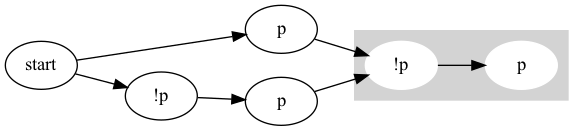
\includegraphics[scale=0.6]{examples/ex2/ex2.gv.png}
        \caption{Timeline representation for formula $\Phi$}
    \end{figure}
    
    $\Psi =$ 
    
   \begin{figure}
        \centering
        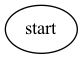
\includegraphics[scale=0.6]{examples/ex3/ex3.gv.png}
        \caption{Timeline representation for formula $\Psi$}
    \end{figure}
\end{frame}

\begin{frame}{LTL to Timeline Conversion}
    Our contribution: an algorithm and a tool that converts any LTL formula into its corresponding timeline
    \begin{itemize}
        \item LTL to state-based \Buchi Automata (BA)
        \item BA to $\omega$-regular expression
        \item Heuristics based $\omega$-regular expression simplification
        \item $\omega$-regular expression to timeline
    \end{itemize}
    \begin{figure}
        \centering
        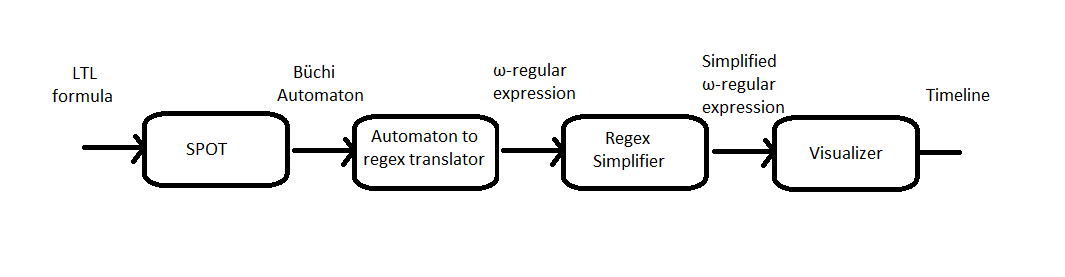
\includegraphics[scale=0.45]{img/algo-flowchart.png}
        %\caption{Caption}
        \label{fig:my_label}
    \end{figure}
\end{frame}

\begin{frame}{LTL to state-based \Buchi Automata (BA)}
    \Buchi Automata: the normal automata you know, except for the accepting condition
    
    \begin{figure}
        \centering
        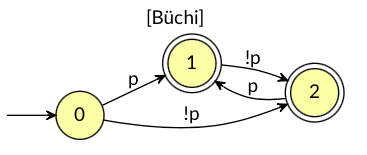
\includegraphics[scale=0.5]{img/buchi-ex.png}
        \caption{Example \Buchi Automata for $\alwaysf ((p \wedge \nexttf \neg p) \vee (\neg p \wedge \nexttf p))$}
    \end{figure}

    This step is very well-studied \cite{Dur22} and our tool uses \textit{Spot}.
\end{frame}

\begin{frame}{BA to $\omega$-regular expression}
    \begin{definition}{Regular expression \& $\omega$-regular expression}
        \begin{align*}
            A & ::= \epsilon \mid \emptyset \mid p (\in \Sigma) \mid AA \mid A + A \mid A^* \\
            B & ::= A^{\omega} \mid AB \mid B + B
        \end{align*}
        Our $\Sigma$ is the set of propositional logic formula.
    \end{definition}

    \begin{definition}
        $A_{(s, f)}^0$ represents the regular expression that corresponds to all paths from state $s$ reaching state $f$ for the first time

        $A_{(s, f)}^1$ represents the regular expression that corresponds to all paths from state $s$ reaching state $f$
    \end{definition}
\end{frame}

\begin{frame}{BA to $\omega$-regular expression, cont}
    \[
        B = \bigplus_{f \in F} A_{(s, f)}^0 (A_{(f, f)}^1)^{\omega}
    \]
    \begin{example}
        \begin{figure}
        \centering
        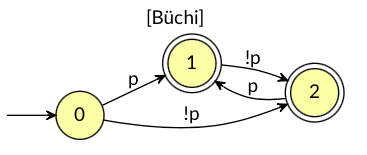
\includegraphics[scale=0.5]{img/buchi-ex.png}
        \caption{Example \Buchi Automata for $\alwaysf ((p \wedge \nexttf \neg p) \vee (\neg p \wedge \nexttf p))$}
    \end{figure}
    Generated $\omega$-regular expression:
    \[
        (p(!pp)^{\omega}) + (!p(p!p)^{\omega})
    \]
    \end{example}
\end{frame}

\begin{frame}{Heuristics based $\omega$-regular expression simplification}
    The $\omega$-regular expression generated may not be the ``simplest'' to visualize.
    \begin{alignat*}{2}
        & r_1 + r_1r_2^* && \Longrightarrow r_1r_2^* \\
        & r + r && \Longrightarrow r \\
        & r_1 + r_2^*r_1 && \Longrightarrow r_2^*r_1 \\
        & (r^*)^{\omega} && \Longrightarrow r^{\omega} \\
        & (r_1r_2^*)r_2^{\omega} && \Longrightarrow r_1r_2^{\omega} \\
        & (r_1r_2)r_2^{\omega} && \Longrightarrow r_1r_2^{\omega} \\
        & r^*r^{\omega} && \Longrightarrow r^{\omega} \\
        & rr^{\omega} && \Longrightarrow r^{\omega}
    \end{alignat*}
\end{frame}

\begin{frame}{Heuristics based $\omega$-regular expression simplification, cont}
    \begin{example}
        $\Phi = \alwaysf (a \limplies \evenf (\neg a))$
    \begin{figure}
        \centering
        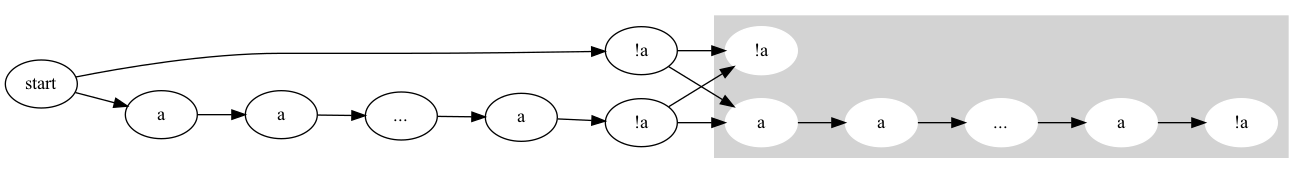
\includegraphics[scale=0.25]{examples/ex9/ex9-unsimplified.gv.png}
        \caption{Timeline for un-simplified $\omega$-regex $((!a) | ((aa^*(!a)))((!a) | ((aa^*(!a)))^{\omega}$}
    \end{figure}
    \begin{figure}
        \centering
        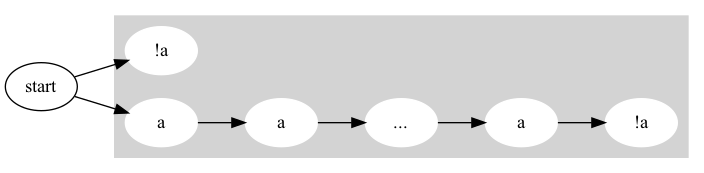
\includegraphics[scale=0.25]{examples/ex9/ex9.gv.png}
        \caption{Timeline for simplified $\omega$-regex $((!a) | ((aa^*(!a)))^{\omega}$}
    \end{figure}
    \end{example}
\end{frame}

\begin{frame}{$\omega$-regular expression to timeline}
    Every $\omega$-regular we generate is the form of 
    \[
        A_1A_2^{\omega} + A_3A_4^{\omega} + \cdots + A_{2n-1}A_{2n}^{\omega}
    \]
    % Every regular expression $A_i$ is visualized as a set of finite length strings.
    \begin{figure}
        \centering
        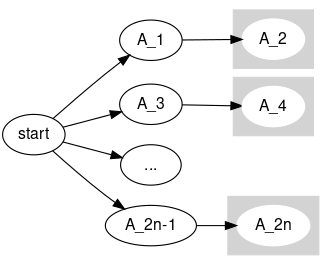
\includegraphics[scale=0.4]{img/timeline.png}
        \caption{Generic timeline representation for arbitrary $\omega$-regular expression}
    \end{figure}
    Out tool uses Graphviz \cite{Ellson2001GraphvizO} for visualization. 
\end{frame}

\begin{frame}{Tool showcase}
    \begin{example}
        $\Phi = \alwaysf (a \limplies \nexttf b)$
        
        ``A message on the controllers monitor indicates when the aircraft has cleared the conflict and control of the aircraft is handed off to the controllers.''\cite{ZR14}

        \begin{figure}
            \centering
            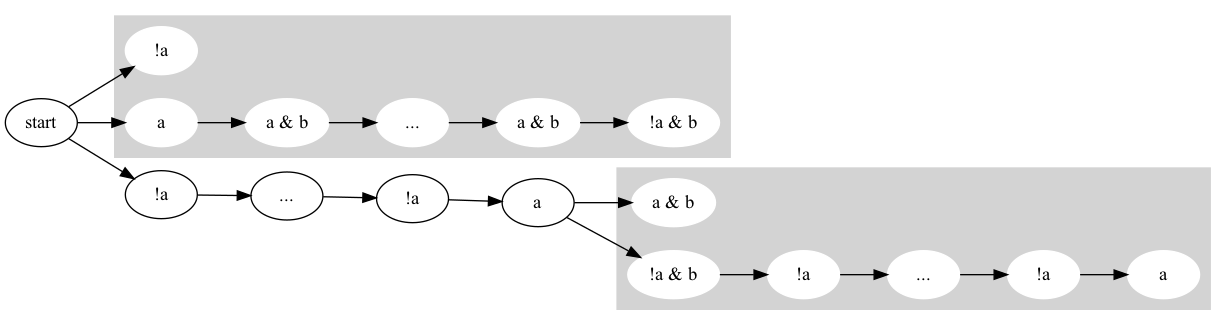
\includegraphics[scale=0.25]{examples/ex4/ex4.gv.png}
            \caption{Timeline for $\Phi = \alwaysf (a \limplies \nexttf b)$}
            \label{fig:my_label}
        \end{figure}
    \end{example}
\end{frame}

\begin{frame}{Tool showcase, cont}
    \begin{example}
        $\Phi = p_2 \land (\evenf (\alwaysf p_0 \strongrelease  1) \weakrelease \nexttf(\alwaysf p_1 \land ((p_0 \liff p_2) \stronguntil \evenf p_0)))$

        A randomly generated LTL formula

        \begin{figure}
            \centering
            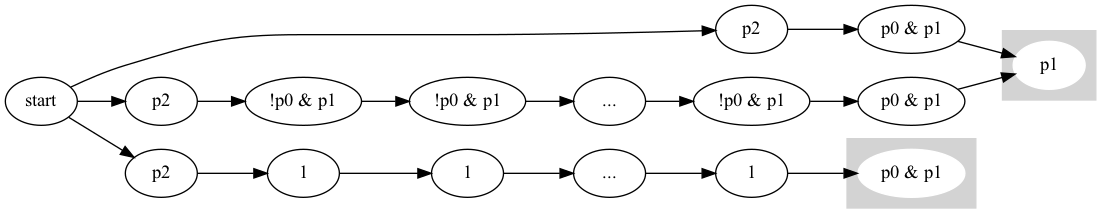
\includegraphics[scale=0.25]{examples/ex13/ex13.gv.png}
            \caption{Timeline for $\Phi = p_2 \land (\evenf (\alwaysf p_0 \strongrelease  1) \weakrelease \nexttf(\alwaysf p_1 \land ((p_0 \liff p_2) \stronguntil \evenf p_0)))$}
        \end{figure}
    \end{example}
\end{frame}

\begin{frame}
    \frametitle{References}
    \printbibliography
\end{frame}

\end{document}